\chapter{روش‌ها و مجموعه‌داده}
\section{بررسی آماری مجموعه داده}

در این پژوهش از مجموعه داده
\lr{PhysioNet}\cite{physionet_hssayeni2020intracranial,hssayeni2020computed}
استفاده شده است که شامل حاشیه‌نویسی برای وظیفه طبقه‌بندی و قطعه‌بندی است. این مجموعه داده  شامل مجموعه‌ای از سی‌تی‌اسکن‌های مغزی است که به صورت عمومی در دسترس است.
تصاویر سی‌تی‌اسکن، از انواع تصاویر سه‌بعدی هستند، همانطور که در 
\autoref{fig:read-ct}
مشخص است،
 با توجه به جهت برش‌های سی‌تی‌اسکن، این تصاویر به سه دسته 
 \lr{Axial}, \lr{Sagital} و \lr{Coronal}
 تقسیم می‌شوند.
\begin{figure}[H]
\centering
\includegraphics[width=1.0\linewidth]{"Images/Chapter2/read CT"}
\caption{خوانش‌های متفاوت از تصاویر سی‌تی‌اسکن
\cite{kaggleCTScansDICOM}}
\label{fig:read-ct}
\end{figure}
 
مجموعه‌داده 
\lr{PhysioNet}
 شامل 82 سی‌تی‌اسکن با برش‌‌های 
\lr{Axial}
است که بین فوریه و آگوست 2018 از بیمارستان آموزشی 
\lr{Al Hilla }
 در عراق جمع‌آوری شده است. این اسکن‌ها شامل طیف وسیعی از بیماران هستند که از یک روز تا 72 سال سن دارند و میانگین سن آنها 
 $27.8 \pm 19.5$
 سال است. تنوع سنی این مجموعه داده بر مقیاس، شکل جمجمه و بافت مغز در سی‌تی‌اسکن تأثیر می‌گذارد، عاملی که می‌تواند عملکرد مدل‌های یادگیری عمیق برای تشخیص و قطعه‌بندی خونریزی درون جمجمه‌ای را تحت تأثیر قرار دهد. توزیع جنسیت در ای نمجموعه‌داده به گونه‌ای است که 56\%  بیماران مرد و 44\% آنها زن هستند.
82 بیماری که در این مجموعه داده وجود دارد که 7 مورد از آنها طی قرایند حاشیه‌نویسی گم شده‌اند و از بین 75 بیمار موجود، 36 نفر دارای خونریزی درون‌جمجمه‌ای تشخیص داده شدند.
\autoref{fig:ch2-slice-number}
نمودار مروبط به تعداد برش‌های هر بیمار در این مجمموعه‌داده است؛ تصاویر سی‌تی‌اسکن موجود در این مجموعه داده،  به طور متوسط شامل 34 برش با ضخامت برش 5 میلی‌متر دارند و در مجموع 2814 برش در این مجموعه‌داده وجود دارد. 
\begin{figure}[H]
\centering
\includegraphics[width=1.0\linewidth]{"Images/Chapter2/Slice number"}
\caption{‌تعداد برش‌های بیماران بر اساس شناسه اختصاصی آنها}
\label{fig:ch2-slice-number}
\end{figure}

با این حال، این مجموعه داده به دلیل عدم توازن در سطح برش شناخته می‌شود، زیرا تنها 318 برش دارای خونریزی هستند در حالی که بقیه 2496 برش سالم هستند. در این مجموعه داده، 24 برش شامل زیرگروه
 \lr{IVH}،
  73 برش شامل زیرگروه
 \lr{CPH}، 
  18 برش شامل زیرگروه
 \lr{SDH}،
173 برش شامل زیرگروه
 \lr{EDH} 
 و 56 برش شامل زیرگروه 
 \lr{SDH}
هستند. با توجه به تفاوت شکل انواع زیرگروه‌های خونریزی و محل وقوع آنها، این ارقام نشان دهنده عدم وجود تعداد برش کافی برای بعضی از انواع زیرگروه‌های است.
در این مجموعه‌داده، برش‌های سی‌تی‌اسکن توسط دو پرتوشناس بررسی شده‌است و هر برش سی‌تی‌اسکن از نظر وجود خونریزی یا شکستگی توسط آنها بررسی و برچسب‌گذاری شده است. در ادامه سی‌تی‌اسکن‌های دو بیمار، به علت کیفیت ضعیف تصاویر و به توصیه پرتوشناس‌ها حذف شدند\cite{kyung2022improved}.

\autoref{fig: ch2-distribution}
نمودارهای توزیع بیمارمحور و برش‌محور مجموعه‌داده را نمایش می‌دهد؛ همانطور که از ‎\autoref{fig: ch2-patient distrbiution}‎ مشخص است در بررسی بیمار‌محور این مجموعه‌داده، عدم توازن دیده نمی‌شود اما در بررسی برش‌محور، همانطور که در ‎\autoref{fig: ch2-slice distribution}‎ 
مشخص است، عدم توازن شدیدی در تعداد برش‌های دارای خونریزی وجود دارد که این مسئله آموزش مدل‌های شبکه عصبی را با چالش مواجه می‌کند.
 \begin{figure}[ht]
		\centering % <-- added
		\begin{subfigure}{0.45\textwidth}
			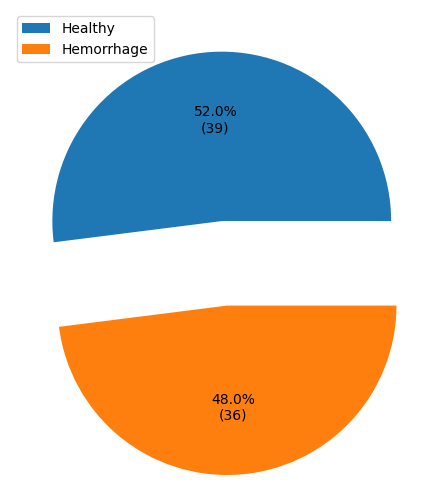
\includegraphics[width=\linewidth]{Images/Chapter2/patient distrbiution.png}
			\caption{}
			\label{fig: ch2-patient distrbiution}
		\end{subfigure}\hfil % <-- added
		\begin{subfigure}{0.45\textwidth}
			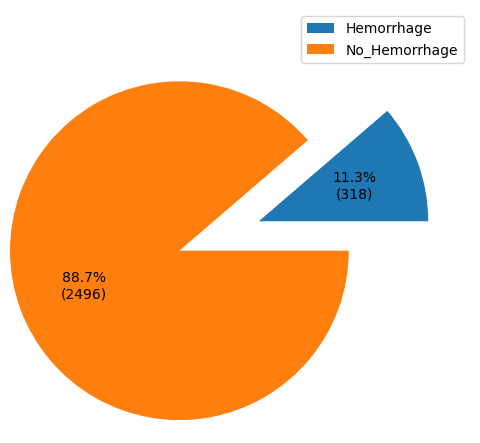
\includegraphics[width=\linewidth,]{Images/Chapter2/slice distribution.png}
			\caption{}
			\label{fig: ch2-slice distribution}
		\end{subfigure}
		\caption{توزیع بیماران و برش‌ها در مجموعه داده 
		\lr{PhysioNet}}
		\label{fig: ch2-distribution}
\end{figure} 

 علاوه بر وجود عدم توازن در حالت برش‌محور، عدم توازن شدیدی در قطعه‌بندی نواحی دارای خونریزی نسبت به نواحی سالم در برش‌های دارای خونریزی وجود دارد که به موجب آن در یک تصویر با ابعاد
$512\times512$،
به صورت میانگین نزدیک به 2000 پیکسل
\LTRfootnote{Pixel}
دارای خونریزی درون‌جمجمه‌ای وجود دارد که این مسئله آموزش مدل‌های شبکه عصبی را به منظور وظیفه قطعه‌بندی با چالش بسیار جدی مواجه می‌کند. 
\autoref{fig: ch2-slice hist}
نشان‌دهنده توزیع نرمال‌شده 
\LTRfootnote{Normalized}
مقدار پیکسل‌های برش‌های سالم و برش‌های دارای خونریزی می‌باشد، با توجه به
\autoref{fig: ch2-slice hist whole}، 
اکثر پیکسل‌های تصاویر مقداری نزدیک به 
$-1000$
و نقطه بیشینه محلی بعدی برای این نمودار توزیع، در نزدیک مقادیر 30 می‌باشد که این مقادیر به نسبت پیکسل‌ها با مقادیر نزدیک به 
$-1000$
خیلی کمتر می‌باشد.


 \begin{figure}[ht]
		\centering % <-- added
		\begin{subfigure}{0.45\textwidth}
			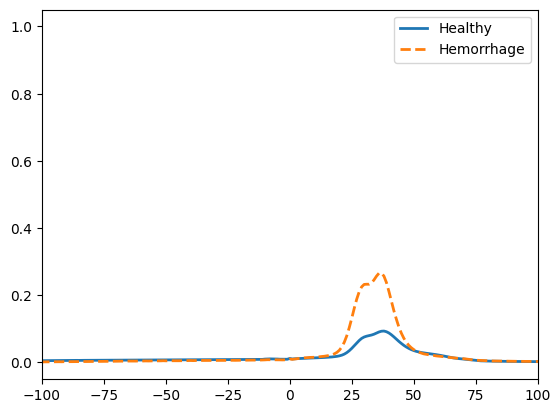
\includegraphics[width=\linewidth]{Images/Chapter2/Pixel histogram.png}
			\caption{}
			\label{fig: ch2-slice hist whole}
		\end{subfigure}\hfil % <-- added
		\begin{subfigure}{0.45\textwidth}
			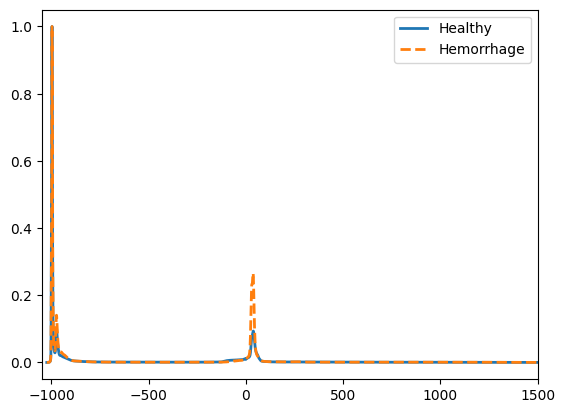
\includegraphics[width=\linewidth,]{Images/Chapter2/Pixel histogram lim.png}
			\caption{}
			\label{fig: ch2-slice hist lim}
		\end{subfigure}
		\caption{توزیع پیکسلی برش‌ها برای برش‌های داداری خونریزی در مقال برش‌های سالم}
		\label{fig: ch2-slice hist}
\end{figure} 

\autoref{fig:ch2-pixel-hist-ich-vs-healthy}
نمایش‌دهنده توزیع پیکسل‌های دارای خونریزی و تمام پیکسل‌های تصاویر رادیوگرافی می‌باشد که در محدوده بین 
$-100$
تا 
$100$
واقع شده است و نسبت به مقادیر همین بازه نرمال گشته است. همانطور که از این دو نمودار مشخص است، مقادیر مربوط به ضایعه خونریزی،‌مقادر کمی از مقادیر بقیه بافت‌های مغز روشن‌تر است اما همپوشانی این دو نمودار نشان می‌دهد که تشخیص خونریزی درون‌جمجمه‌ای تنها با استفاده از مقدار پیکسلی آن بسیار دشوار می‌باشد و نیاز هست تا از شبکه‌هایی استفاده شود تا به اشکال موجود در تصویر نیز حساسیت داشته باشند.


\begin{figure}[H]
\centering
\includegraphics[width=1.0\linewidth]{"Images/Chapter2/pixel hist ich vs healthy"}
\caption{توزیع نرمال‌شده پیکسل‌های دارای خونریزی درمقابل تمام پیکسل‌های تصاویر}
\label{fig:ch2-pixel-hist-ich-vs-healthy}
\end{figure}


\autoref{fig:ch2-slice-number}
توزیع خونریزی درون‌جمجمه‌ای را بر اساس شماره برش در تصویر سی‌تی‌اسکن نشان می‌دهد که بر اساس آن مشخص است به ازای بعضی از شماره برش‌ها خونریزی درون‌جمجمه‌ای وجود ندارد و این برش‌ها از اهمیت کمتری برای مدل‌های یادگیری ماشین برخوردار هستند.

\begin{figure}[H]
\centering
\includegraphics[width=1.0\linewidth]{"Images/Chapter2/slice hist"}
\caption{توزیع خونریزی بر اساس برش‌ها}
\label{fig:ch2-slice-hist}
\end{figure}


مجموعه داده PhysioNet به عنوان یک معیار مهم برای توسعه و آزمون الگوریتم‌های تشخیص و قطعه‌بندی ICH خدمت می‌کند. مطالعه همراه از یک مدل یادگیری عمیق، به‌ویژه U-Net، برای خودکارسازی قطعه‌بندی مناطق ICH در برش‌های CT استفاده کرده است. تنوع جمعیتی این مجموعه داده، همراه با چالش‌های ناشی از عدم توازن در سطح برش، محیطی قوی برای ارزیابی اثربخشی الگوریتم‌های قطعه‌بندی فراهم می‌کند.
دسترسی این مجموعه داده در PhysioNet اهمیت آن را در تقویت تحقیقات باز و همکاری در جامعه پزشکی برجسته می‌کند. این مجموعه داده نیاز به مجموعه‌های داده استاندارد و عمومی در دسترس را که می‌توانند برای مقایسه و اعتبارسنجی روش‌های مختلف یادگیری ماشین استفاده شوند، به‌ویژه در زمینه‌های حیاتی مانند تشخیص ICH که تشخیص به موقع و دقیق می‌تواند نجات‌بخش باشد، برآورده می‌کند.
